%iffalse
\let\negmedspace\undefined
\let\negthickspace\undefined
\documentclass[journal,12pt,twocolumn]{IEEEtran}
\usepackage{cite}
\usepackage{amsmath,amssymb,amsfonts,amsthm}
\usepackage{algorithmic}
\usepackage{graphicx}
\usepackage{textcomp}
\usepackage{xcolor}
\usepackage{txfonts}
\usepackage{listings}
\usepackage{enumitem}
\usepackage{mathtools}
\usepackage{gensymb}
\usepackage{comment}
\usepackage[breaklinks=true]{hyperref}
\usepackage{tkz-euclide}
\usepackage{listings}
\usepackage{gvv}                                        
%\def\inputGnumericTable{}                                
\usepackage[latin1]{inputenc}                                
\usepackage{color}                                            
\usepackage{array}                                            
\usepackage{longtable}                                      
\usepackage{calc}                                            
\usepackage{multirow}                                        
\usepackage{hhline}                                          
\usepackage{ifthen}                                          
\usepackage{lscape}
\usepackage{tabularx}
\usepackage{array}
\usepackage{float}
\usepackage{multicol}


\newtheorem{theorem}{Theorem}[section]
\newtheorem{problem}{Problem}
\newtheorem{proposition}{Proposition}[section]
\newtheorem{lemma}{Lemma}[section]
\newtheorem{corollary}[theorem]{Corollary}
\newtheorem{example}{Example}[section]
\newtheorem{definition}[problem]{Definition}
\newcommand{\BEQA}{\begin{eqnarray}}
\newcommand{\EEQA}{\end{eqnarray}}
\newcommand{\define}{\stackrel{\triangle}{=}}
\theoremstyle{remark}
\newtheorem{rem}{Remark}

% Marks the beginning of the document
\begin{document}
\bibliographystyle{IEEEtran}
\vspace{3cm}

\title{2007-EE}
\author{ee24btech11064 - Harshil Rathan}
\maketitle
\newpage
\bigskip

\renewcommand{\thefigure}{\theenumi}
`\renewcommand{\thetable}{\theenumi}
\begin{enumerate}
\item The system $\frac{900}{s(s + 1)(s + 9)}$ is to be compensated such that its gain-crossover frequency becomes the same as its uncompensated phase-crossover frequency and provides a $45^\circ$ phase margin. To achieve this, one may use:
\begin{enumerate}
    \item a lag compensator that provides an attenuation of $20dB$ and a phase lag of $45^\circ$ at the frequency of $3\sqrt{3}$ rad/s
    \item  a lag compensator that provides an amplification of $20dB$ and a phase lead of $45^\circ$ at the frequency of $3$ rad/s
    \item  a lag-lead compensator that provides an amplification of $20dB$ and a phase lag of $45^\circ$ at the frequency of $\sqrt{3}$ rad/s
    \item  a lag-lead compensator that provides an attenuation of $20dB$ and a phase lead of $45^\circ$ at the frequency of $3$ rad/s
\end{enumerate}
\item Consider the discrete-time system shown in figure where the impulse response of $G\brak{z}$ is $g\brak{0}=0$, $g\brak{1}=g\brak{2}=1$,  $g\brak{3}=g\brak{4}=\cdots=0$
\begin{figure}[h!]
    \centering
    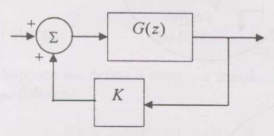
\includegraphics[width=0.7\linewidth]{figs/q36.png}
\end{figure}
This system is stable for range of values of $K$
\begin{multicols}{2}
\begin{enumerate}
    \item $[-1,\frac{1}{2}]$
    \item $[-1,1]$
    \item $[\frac{-1}{2},1]$
    \item $[\frac{-1}{2},2]$
\end{enumerate}
\end{multicols}
\item A signal \(x(t)\) is given by
\[
x(t) =
\begin{cases}
1, & -\frac{T}{4} < t \leq \frac{3T}{4} \\
-1, & \frac{3T}{4} < t \leq \frac{7T}{4} \\
-x(t + T) & \text{(periodic extension)}
\end{cases}
\]

Which among the following gives the fundamental Fourier term of $x\brak{t}$?
\begin{multicols}{2}
\begin{enumerate}
       \item $\frac{4}{\pi}\cos({\frac{\pi t}{T}-\frac{\pi}{4}})$
       \item $\frac{\pi}{4}\cos({\frac{\pi t}{2T}-\frac{\pi}{4}})$
       \item $\frac{4}{\pi}\sin({\frac{\pi t}{T}-\frac{\pi}{4}})$
       \item $\frac{\pi}{4}\sin({\frac{\pi t}{2T}-\frac{\pi}{4}})$
\end{enumerate}
\end{multicols}
\item If the loop gain K of a negative feedback system having a loop transfer function $\frac{K\brak{s+3}}{\brak{s+8}^2}$ is to be adjusted to induce a sustained oscillation then 
\begin{enumerate}
    \item The frequency of this oscillation must be $\frac{4}{\sqrt{3}}$ rad/s
    \item The frequency of this oscillation must be $4$ rad/s
    \item The frequency of this oscillation must be $4$ or $\frac{4}{\sqrt{3}}$ rad/s
    \item such a K does not exist
\end{enumerate}
\item The system shown in figure below 
\begin{figure}[h!]
    \centering
    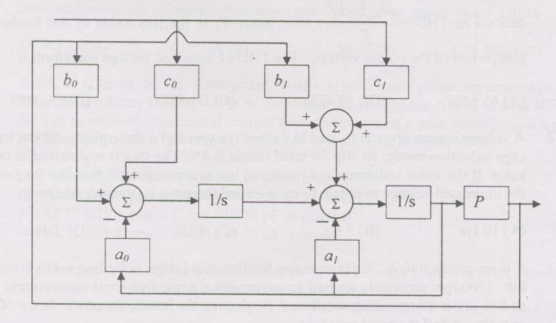
\includegraphics[width=0.7\linewidth]{figs/q39(1).png}
\end{figure}
can be reduced to the form
\begin{figure}[h!]
    \centering
    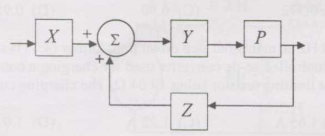
\includegraphics[width=0.7\linewidth]{figs/q39(2).png}
\end{figure}
\begin{enumerate}
    \item $X=c_0s+c_1$, $Y=\frac{1}{s^2+a_0s+a_1}$, $Z=b_0s+b_1$
    \item $X=1$, $Y=\frac{c_0s+c_1}{s^2+a_0s+a_1}$, $Z=b_0s+b_1$
    \item $X=c_1s+c_0$, $Y=\frac{b_1s+b_0}{s^2+a_1s+a_0}$, $Z=1$
    \item $X=c_1s+c_0$, $Y=\frac{1}{s^2+a_1s+a_0}$, $Z=b_1s+b_0$
\end{enumerate}
\item The value of $\oint_{C}\frac{dz}{(1+z^{2})}$ where C is contour $|z-\frac{i}{2}|=1$ is 
\begin{multicols}{2}
\begin{enumerate}
    \item $2\pi i$
    \item $\pi$
    \item $\tan^-{1}{z}$
    \item $\pi i \tan^-{1}{z}$ 
\end{enumerate}
\end{multicols}
\item A single-phase voltage source inverter is controlled in a single pulse-width modulated mode with a pulse width of $150^\circ$ in each half cycle. Total harmonic distortion is defined as $THD=\frac{\sqrt{V_{rms}^2-V_1^2}}{V_1}\times 100$, where $V_1$ is the rms value of the fundamental component of the output voltage. The THD of output ac voltage waveform is 
\begin{multicols}{2}
\begin{enumerate}
    \item $65.65\%$
    \item $48.42\%$
    \item $31.83\%$
    \item $30.49\%$
\end{enumerate}    
\end{multicols}
\item A voltage source inverter is used to control the speed of a three-phase, $50Hz$, squirrel cage induction motor. Its slip for rated torque is $4\%$. The flux is maintained at rated value. If the stator resistance and rotational losses are neglected, then the frequency of the impressed voltage to obtain twice the rated troque at starting should be
\begin{multicols}{2}
\begin{enumerate}
    \item $10Hz$
    \item $5Hz$
    \item $4Hz$
    \item $2Hz$
\end{enumerate}    
\end{multicols}
\item A three-phase, $440V$, $50Hz$ ac mains fed thyristor bridge is feeding a $440 V$dc, $15kW$, $1500$rpm separately excited dc motor with a ripple free continuous current in the dc link under all operating conditions. Neglecting the losses, the power factor of the ac mains at half the rated speed, is 
\begin{multicols}{2}
\begin{enumerate}
    \item $0.354$
    \item $0.372$
    \item $0.90$
    \item $0.955$
\end{enumerate}    
\end{multicols}
\item A single-phase, $230V$, $50$Hz ac mains fed step down transformer $\brak{4:1}$ is supplying power to a half-wave uncontrolled ac-dc converter used for charginga battery $\brak{12Vdc}$ with the series current limiting resistor being $19.04\ohm$, The charging current is
\begin{multicols}{2}
\begin{enumerate}
    \item $2.43A$
    \item $1.65A$
    \item $1.22A$
    \item $1.0A$
\end{enumerate}    
\end{multicols}
\item A three-phase synchronous motor connected to ac mains is runnign at full load and unity power factor. If its shift load is reduced by half, with field current held constant, its new power factor will be 
\begin{enumerate}
    \item unity
    \item leading
    \item lagging
    \item dependent on machine parameters
\end{enumerate}    
\item A $100kVA$, $415V\brak{line}$, star-connected synchronous machine generates rated open circuit voltage of $415V$ at a field current of $15A$. The short circuit armature current at a field current of $10A$ is equal to the rated armature current. The per unit saturated synchronous reactance is 
\begin{multicols}{2}
\begin{enumerate}
    \item $1.731$
    \item $1.5$
    \item $0.666$
    \item $0.577$
\end{enumerate}    
\end{multicols}
\item A three-phase, three-stack, variable reluctance step motor has 20 poles on each rotor ans stator stack. The step angle of this step motor is
\begin{multicols}{2}
\begin{enumerate}
    \item $3^\circ$
    \item $6^\circ$
    \item $9^\circ$
    \item $18^\circ$
\end{enumerate}    
\end{multicols}
\item A single-phase $50$kVA, $250V/500V$ two winding transformer has an efficiency of $95\%$ at full load, unity power factor. If it is reconfigured as $500V/750V$ autotransformer, its efficiency at its new rated load at unity power factor will be 
\begin{multicols}{2}
\begin{enumerate}
  \item $95.752\%$
    \item $97.851\%$
    \item $98.276\%$
    \item $99.241\%$
\end{enumerate}    
\end{multicols}
\item A $230V$(Phase), $50Hz$, three-phase, 4-wire system has a phase sequence ABC. A unity power-factor load of $4kW$ is connected betweem phase A and neutral N. It is desired to achieve zero neutral current through the use fo a pure inductor and a pure capacitor in the other two phases. The value of inductor and capacitor is 
\begin{enumerate}
    \item $72.95$mH in phase C and $139.02\micro$F in phase B
     \item $72.95$mH in phase B and $139.02\micro$F in phase C
      \item $42.12$mH in phase C and $240.79\micro$F in phase B
      \item $42.12$mH in phase B and $240.79\micro$F in phase C
\end{enumerate}
\item The state equation for the current $I_1$ shown in the network shown below in terms of the voltage $V_x$ and the independent source $V$, is given by 
\begin{figure}[h!]
    \centering
    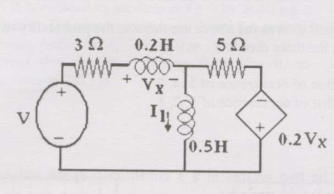
\includegraphics[width=0.7\linewidth]{figs/q50.png}
\end{figure}
\begin{enumerate}
  \item $\frac{dI_i}{dt}=-1.4V_x - 3.75I_i + \frac{5}{4}V$
    \item $\frac{dI_j}{dt}=1.4V_3 - 3.75I_j - \frac{5}{4}V$
    \item $\frac{dI_i}{dt}=-1.4V_s + 3.75I_i + \frac{5}{4}V$
    \item $\frac{dI_j}{dt}=-1.4V_x + 3.75I_t - \frac{5}{4}V$
\end{enumerate}
\item If $u\brak{t}$, $r\brak{t}$ denote the unit step and unit ramp functions respectively and $u\brak{t}*r\brak{t}$ their convolution, then the function $u\brak{t+1}*r\brak{t-2}$ is given by 
\begin{multicols}{2}
\begin{enumerate}
  \item $\brak{\frac{1}{2}}\brak{t-1}\brak{t-2}$
    \item $\brak{\frac{1}{2}}\brak{t-1}\brak{t-2}$
    \item $\brak{\frac{1}{2}}\brak{t-1}^2 u\brak{t-1}$
    \item none of the above
\end{enumerate}    
\end{multicols}
\end{enumerate}
\end{document}
